\chapter{結果と考察}
本章では,シミュレーション,評価実験,アンケートの結果とその考察について述べる.

\section{シミュレーション結果と考察}
シミュレーションの結果,Pillowでは一定時間経過後のリマインダーが24回,ソースコード変更量の検知が32回呼び出され,Pipenvでは一定時間経過後のリマインダーが24回,ソースコード変更量の検知が451回呼び出されることがわかった.
Pipenvのシミュレーション結果を図\ref{sim1},Pillowのシミュレーション結果を図\ref{sim2}に示す.
水色の折れ線がドキュメントのコミット数,オレンジ色の折れ線がソースコードのコミット数,紫色の点がC2の呼び出し,緑色の点がC4の呼び出しを表す.
C3については呼び出しがなかった.
また,シミュレーション結果を図に表す時,各機能の呼び出しを日単位でまとめているため,実際の呼び出し回数より少なく表示されている.

\begin{figure}[H]
    \centering
    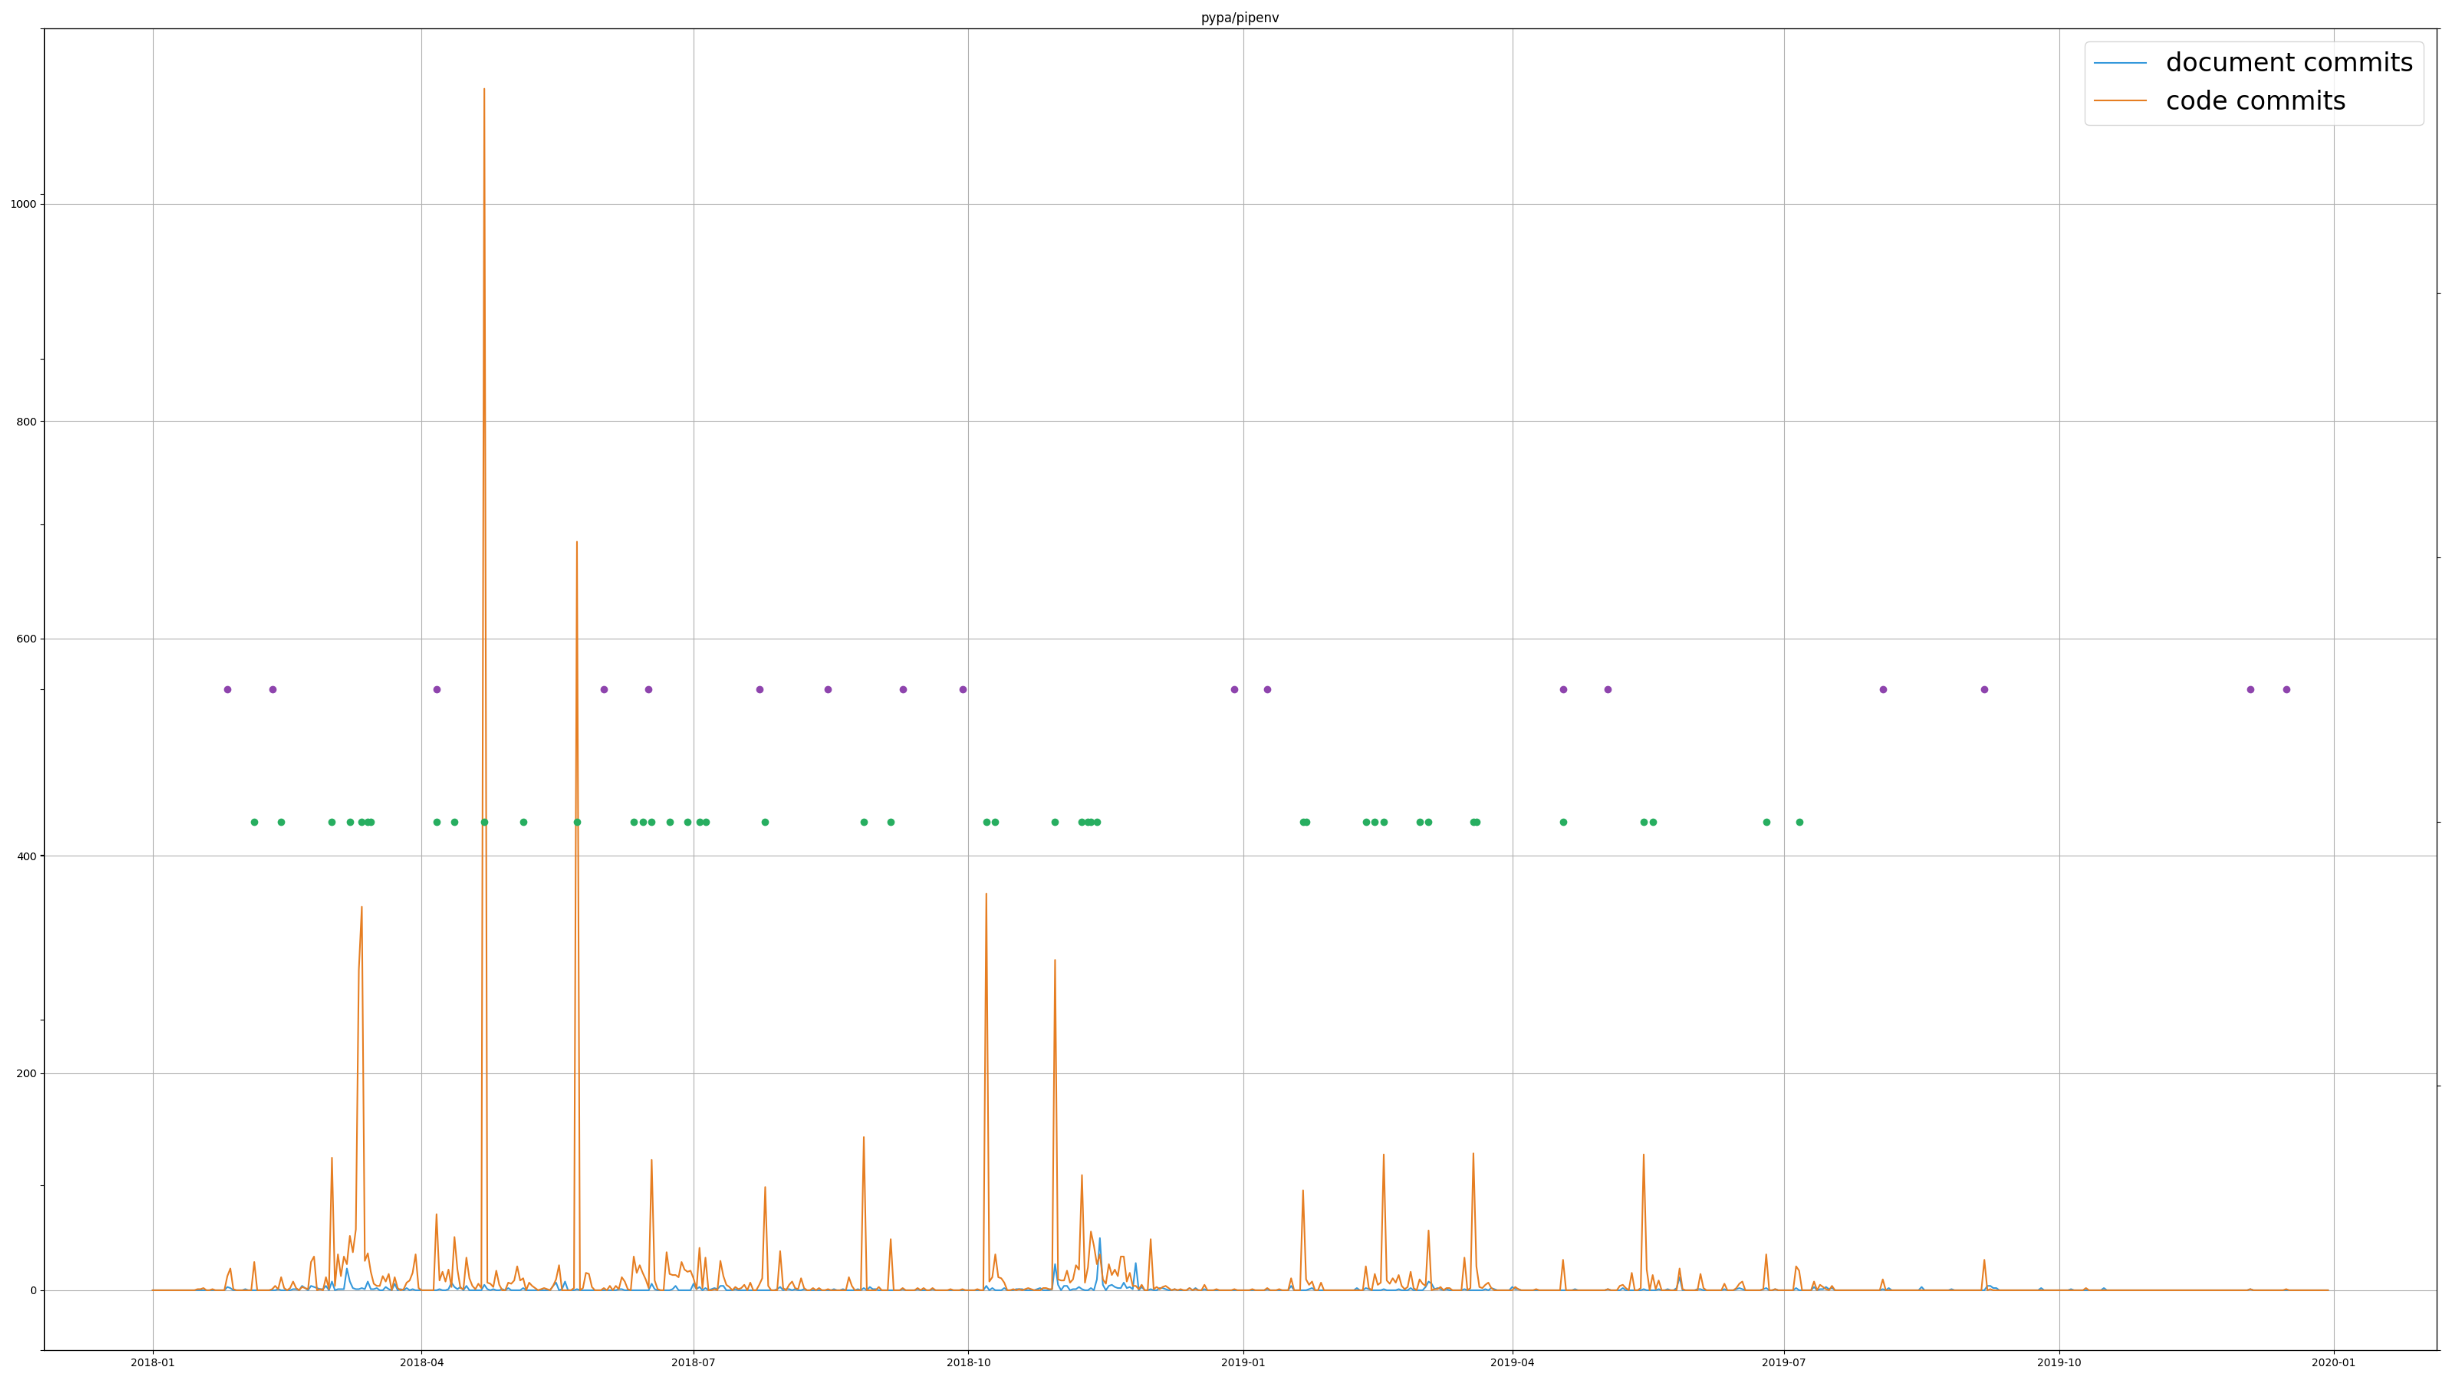
\includegraphics[width=14cm]{images/sim1.png}
    \caption{Pipenvのシミュレーション結果}
    \label{sim1}
\end{figure}

\begin{figure}[H]
    \centering
    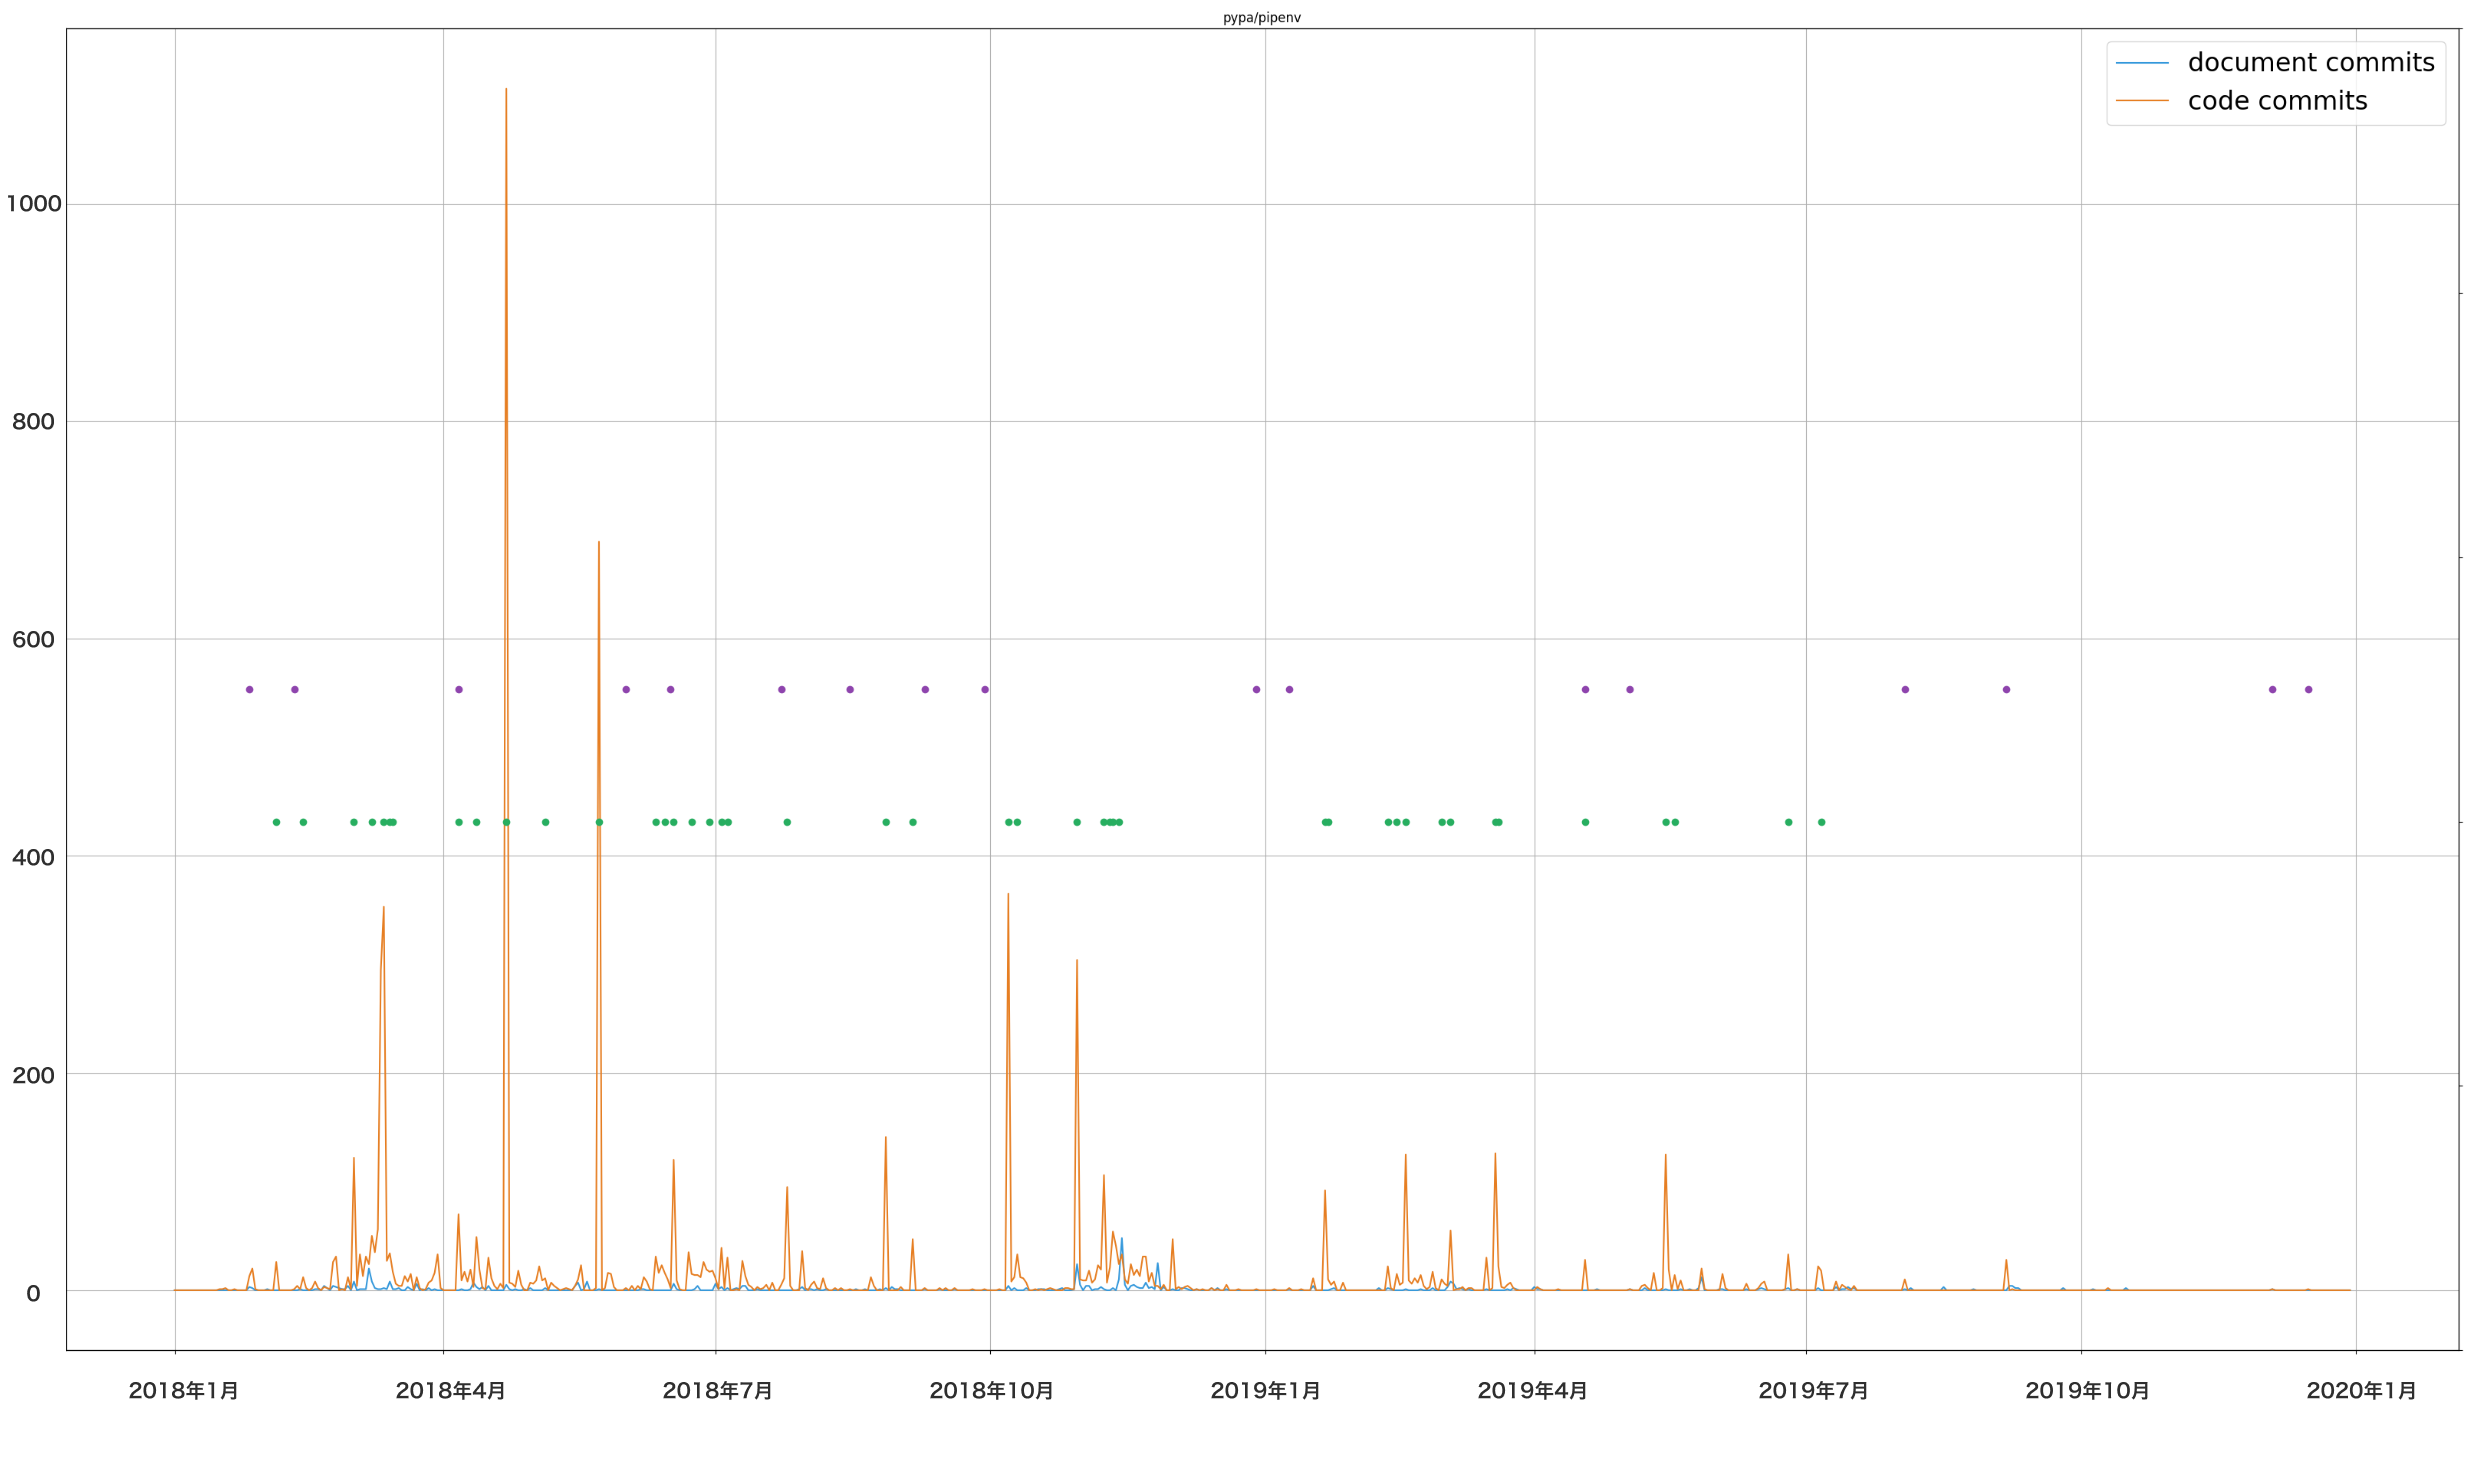
\includegraphics[width=14cm]{images/sim2.png}
    \caption{Pillowのシミュレーション結果}
    \label{sim2}
\end{figure}

Pillowのシミュレーション結果において,図\ref{simpillow}の2014年2月〜2014年10月のコミット数に着目すると,他の時期と比較して数多くのソースコードのコミットがされていることがわかる.
このような時期はソフトウェアとドキュメントの乖離が起きやすく,適切な通知を行うことで,ドキュメントとソースコードが乖離していた場合に,乖離が抑制できることが期待できる.
\begin{figure}[H]
    \centering
    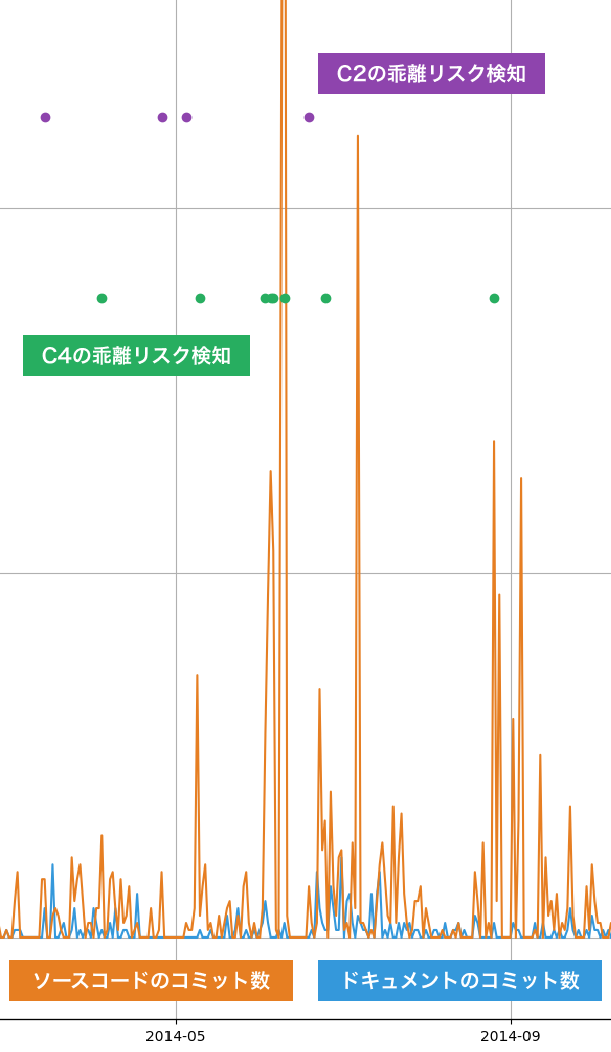
\includegraphics[width=10cm]{images/pillow.png}
    \caption{積極的な開発が行われている時期のPillowのシミュレーション結果}
    \label{simpillow}
\end{figure}

一方で,図\ref{simpipenv}に着目すると,Pipenvでは2019年以降に積極的な開発が行われていないため,ドキュメントとソースコードのコミット数が減少傾向にあることがわかる.
積極的な開発が行われていない時期では,機能追加のためにドキュメントが更新されることはあまりないことからドキュメントとソースコードの乖離が起こることは少ないと考えられるため,このような時期は通知を出さないように改良する必要があることが判明した.
\begin{figure}[H]
    \centering
    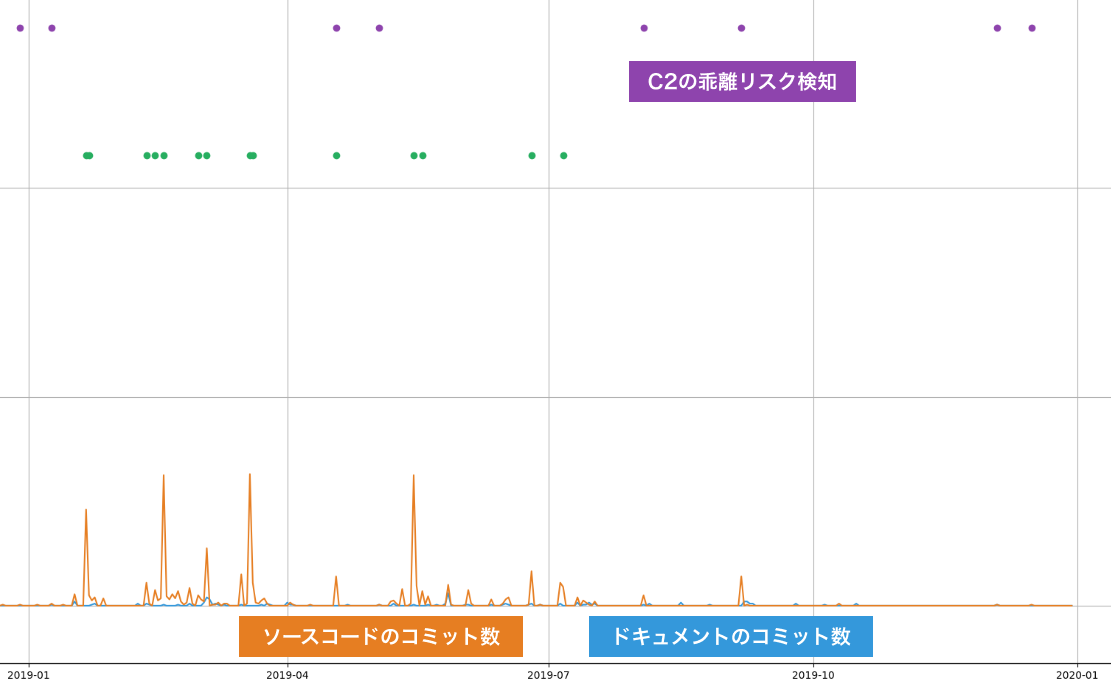
\includegraphics[width=12cm]{images/pipenv.png}
    \caption{積極的な開発が行われていない時期のPipenvのシミュレーション結果}
    \label{simpipenv}
\end{figure}

図\ref{time}は,PillowとPipenvにおいて,乖離リスクが解消されるまでに要した時間を表すグラフである.
ほとんどの場合において,提案ツールを使用しなかった場合,1日以内に乖離リスクを解消している様子が見られた.
一方で,1週間〜2週間程度にわたって乖離リスクが解消しないこともあるため,提案ツールを使用することで乖離リスクを解消することが期待できると考えられる.
\begin{figure}[H]
    \centering
    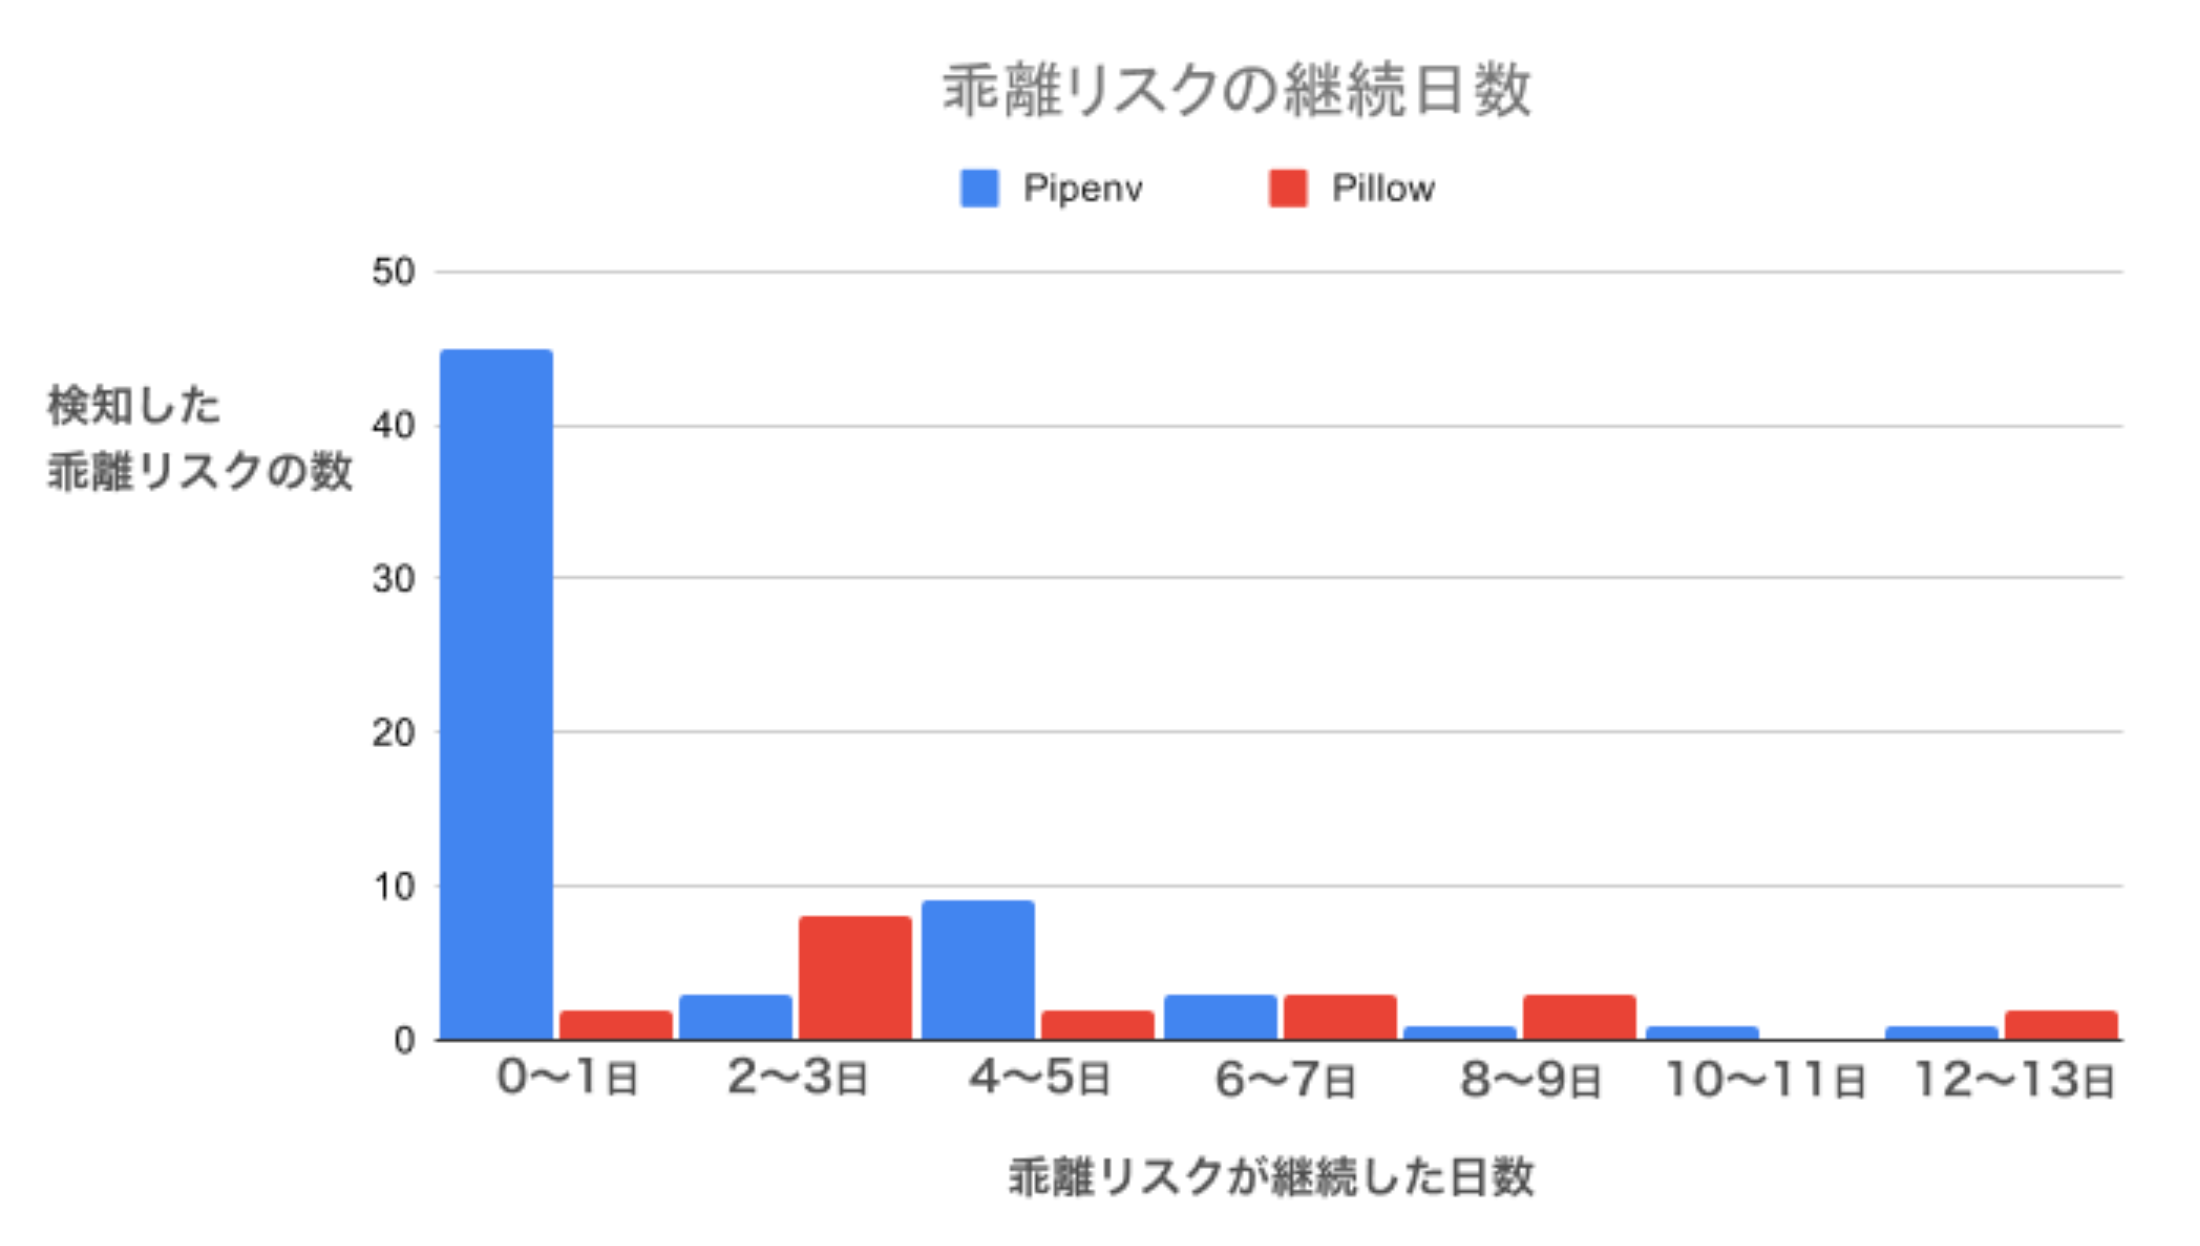
\includegraphics[width=12cm]{images/time.png}
    \caption{乖離の解消時刻}
    \label{time}
\end{figure}

以上のシミュレーション結果より,ドキュメントとソースコードの乖離リスクが検知されたときに通知を出すことで,乖離の抑制に役立つ可能性があることが判明した.
一方で,精度の高い検知を行うためには,さらなる改善を加えないといけないことがわかった.
また,様々なプロジェクトでシミュレーションを行うことのできるシミュレータの改善や,プロジェクト規模に合わせた各種パラメータの自動調整などをする必要があると考える.


\section{実験結果と考察}
\ref{plan}節で示した実験計画に従って評価実験を行った.
以下では,実験協力者2名について,それぞれのタスクの取り組みや,ドキュメントとソースコードの乖離検知をしたときの行動を詳細にまとめる.

\subsection{前半に提案ツールを使用した実験協力者}
前半に提案ツールを使用した実験協力者(以下,実験協力者Aと呼ぶ)の行動と乖離検知の流れを図\ref{usera}に示す.
実験協力者Aは,事前説明に35分,前半タスクに54分,後半タスクに41分の時間を要した.
\begin{figure}[H]
    \centering
    \includegraphics[width=14cm]{images/usera.png}
    \caption{前半に提案ツールを使用した実験協力者の行動と乖離検知の流れ}
    \label{usera}
\end{figure}

実験協力者Aは,既存の機能に新たなバリデーションを追加するタスク1では,ドキュメントを更新せずにソースコードの追加のみを行っていた.
このとき,提案ツールでは\ref{c1}で示したとおり,ドキュメントとソースコードのoperationIdのみを用いて乖離検知を行っているため,
既存の機能に新たなバリデーションを追加し,新規エラーメッセージを返す機能については乖離検知を行うことができない.
そのため,タスク1で変更されることのなかったドキュメントに対して,通知を送ることはなかった.
次に,新たな機能を作成するタスク2を終えたときに,提案ツールが乖離検知を行ったため,実験協力者Aに「[C1]: ドキュメントに無い機能であるget\_users を作成しています」と通知を送った.
図\ref{notification1}は実際に実験協力者Aに通知を行った時のメッセージである.
実験協力者Aは,通知を受け取った後,タスク1とタスク2で生じたドキュメントとソースコードの乖離を修正したため,乖離が抑制された.

\begin{figure}[H]
    \centering
    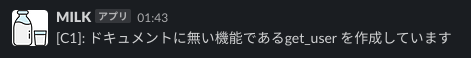
\includegraphics[width=10cm]{images/notification1.png}
    \caption{乖離検知をしたときに実験協力者Aに通知を送ったときのメッセージ}
    \label{notification1}
\end{figure}

その後の後半タスクでは,前半に乖離検知の通知を受け取ったことを受けて,タスクに取り組むときは,ドキュメントとソースコードの両方を追加・修正しており,
ドキュメントとソースコードが乖離することはなかった.

\subsection{後半に提案ツールを使用した実験協力者}
後半に提案ツールを使用した実験協力者(以下,実験協力者Bと呼ぶ)の行動と乖離検知の流れを図\ref{userb}に示す.
実験協力者Bは,事前説明に40分,前半タスクに31分,後半タスクに23分の時間を要した.
\begin{figure}[H]
    \centering
    \includegraphics[width=14cm]{images/userb.png}
    \caption{後半に提案ツールを使用した実験協力者の行動と乖離検知の流れ}
    \label{userb}
\end{figure}

実験協力者Bは,前半タスクをこなす間,一度もドキュメントに触れることなくソースコードの追加を行っていた.
後半タスク開始時に,ドキュメントとソースコードの乖離検知が行われたため,実験協力者Bに「[C1]: ドキュメントに無い機能であるget\_user get\_users\_child を作成しています」と通知を送った.
図\ref{notification2}は実際に実験協力者Bに通知を行った時のメッセージである.

\begin{figure}[H]
    \centering
    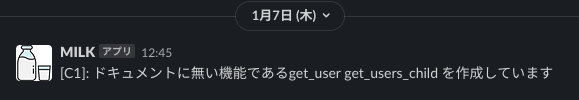
\includegraphics[width=10cm]{images/notification2.png}
    \caption{乖離検知をしたときに実験協力者Aに通知を送ったときのメッセージ}
    \label{notification2}
\end{figure}

ここで,タスク6を開始する前に,実験協力者Bはドキュメントの更新を行ったため,タスク1〜タスク5で生じたドキュメントとソースコードの乖離が抑制された.
その後,後半タスクが終了するまでドキュメントとソースコードの変更を同時に行った.

\subsection{実験結果の考察}
上記では実験協力者2名について,それぞれのタスクの取り組みや,ドキュメントとソースコードの乖離検知をしたときの行動を詳細にまとめた.
2名とも,乖離検知の通知を受け取った直後に,ドキュメントの修正を行っており,全タスク終了時にはドキュメントとソースコードが乖離することはなかった.
このことから,RESTful APIの開発において,提案ツールはドキュメントとソースコードの乖離抑制に一定の効果が見込めることが判明した.
一方で,実験協力者Aのタスク1において,バリデーションを修正したがドキュメントを更新しなかったことについて,
乖離を検知できなかったため,提案ツールの性能を向上させる必要があると考えられる.

\section{アンケート結果と考察}
実施したアンケートを付録\ref{survey}に示す.
実験協力者2名に対し,Slackからの通知を受け取ったことで,ドキュメントを更新しないといけないと感じたかという質問に対し,1名が「とても思った」,1名が「やや思った」と回答した.
回答結果を図\ref{q1}に示す.
\begin{figure}[H]
    \centering
    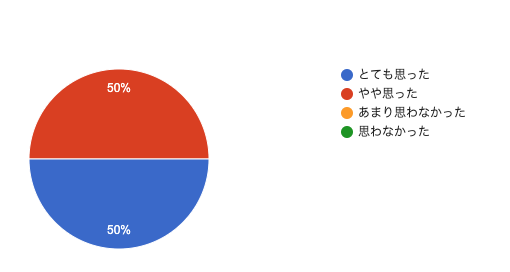
\includegraphics[width=10cm]{images/q1.png}
    \caption{アンケート結果: Slackからの通知を受け取ったことで,ドキュメントを更新しないといけないと感じたか}
    \label{q1}
\end{figure}

また,ドキュメントの更新を忘れてしまったとき,通知は必要だと感じるかという質問に対し,2名が必要であると回答した.
回答結果を図\ref{q2}に示す.
\begin{figure}[H]
    \centering
    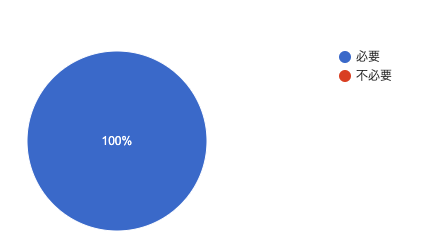
\includegraphics[width=10cm]{images/q2.png}
    \caption{アンケート結果: ドキュメントの更新を忘れてしまったとき,通知は必要だと感じるか}
    \label{q2}
\end{figure}

Slackから受け取った通知内容で改善して欲しいところはあるかという質問に対して,以下のような回答を得た.
\begin{itemize}
    \item 通知内容が簡素に感じた
    \item もっと詳細を教えて欲しい
\end{itemize}

以上のアンケート結果より,提案ツールはドキュメントとソースコードの乖離の抑制に効果を感じていることがわかった.
一方で,通知内容を改善し,開発者に親しみやすいように改良を加えることで,より使いやすいツールになることが判明した.